\documentclass[tikz,border=6pt]{standalone}
\usepackage{pgfplots}
\pgfplotsset{compat=1.18}
\usepgfplotslibrary{colormaps}
\usetikzlibrary{arrows, arrows.meta, calc}
\usetikzlibrary{decorations.markings}


\usepackage{amssymb,amsmath,mathtools}

\usepackage[T1]{fontenc}
\usepackage[utf8]{inputenc}
\usepackage{newpxtext,newpxmath}
\usepackage{sectsty}

\newcommand{\Arg}{\textrm{Arg}}

\renewcommand{\Re}{\operatorname{\mathrm{Re}}}
\renewcommand{\Im}{\operatorname{\mathrm{Im}}}

\begin{document}
	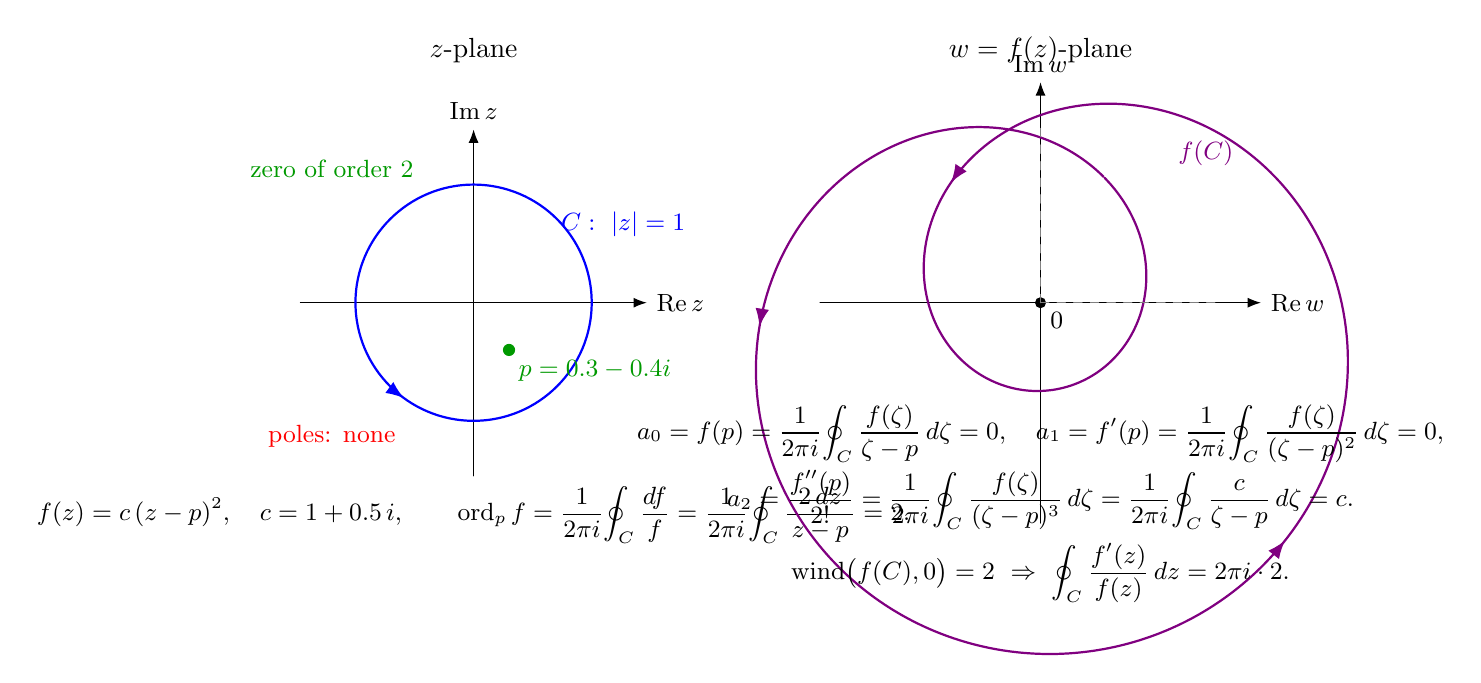
\begin{tikzpicture}[>=Latex, line cap=round, line join=round, font=\small]
		
		%========================
		% Left: z-plane
		%========================
		\begin{scope}[shift={(0,0)}]
			\node[font=\normalsize] at (0,3.2) {$z$-plane};
			% axes
			\draw[->] (-2.2,0)--(2.2,0) node[right] {$\Re z$};
			\draw[->] (0,-2.2)--(0,2.2) node[above] {$\Im z$};
			
			% unit circle C (positively oriented) -- radius 1.5 for visibility
			\draw[blue,thick,postaction={decorate},
			decoration={markings, mark=at position 0.65 with {\arrow{>}}}]
			(0,0) circle (1.5);
			\node[blue] at (1.9,1.0) {$C:\ |z|=1$};
			
			% zero at p (order 2), choose concrete p inside C
			\fill[green!60!black] (0.45,-0.6) circle(2.2pt) node[below right] {$p=0.3-0.4i$};
			\node[green!60!black] at (-1.8,1.7) {zero of order $2$};
			\node[red] at (-1.8,-1.7) {poles: none};
			
			% function label + order via winding form (note: c cancels in df/f)
			\node[align=left] at (0,-2.7) {$\displaystyle
				f(z)=c\,(z-p)^{2},\quad c=1+0.5\,i,\qquad
				\operatorname{ord}_{p} f
				=\frac{1}{2\pi i}\!\oint_C \frac{df}{f}
				=\frac{1}{2\pi i}\!\oint_C \frac{2\,dz}{\,z-p\,}=2.$};
		\end{scope}
		
		%========================
		% Right: w-plane = f(z)-plane
		%========================
		\begin{scope}[shift={(7.2,0)}]
			\node[font=\normalsize] at (0,3.2) {$w=f(z)$-plane};
			% axes
			\draw[->] (-2.8,0)--(2.8,0) node[right] {$\Re w$};
			\draw[->] (0,-2.8)--(0,2.8) node[above] {$\Im w$};
			
			% origin
			\fill (0,0) circle(2pt) node[below right] {$0$};
			
			% image curve f(C): z = 1.5 e^{it} -> w = c (z-p)^2
			% Let u = 1.5 cos t - 0.3, v = 1.5 sin t + 0.4 (so z-p = u + i v).
			% With c = a+ib = 1 + 0.5 i and (u+iv)^2 = (u^2 - v^2) + i(2uv),
			% Re w = a(u^2 - v^2) - b(2uv),  Im w = a(2uv) + b(u^2 - v^2).
			\draw[violet,thick,
			postaction={decorate},
			decoration={markings,
				mark=at position 0.18 with {\arrow{>}},
				mark=at position 0.48 with {\arrow{>}},
				mark=at position 0.78 with {\arrow{>}}}]
			plot[domain=0:6.283, samples=650]
			({
				( (1.5*cos(\x r)-0.3)^(2) - (1.5*sin(\x r)+0.4)^(2) )
				- 0.5*( 2*(1.5*cos(\x r)-0.3)*(1.5*sin(\x r)+0.4) )
			},
			{
				( 2*(1.5*cos(\x r)-0.3)*(1.5*sin(\x r)+0.4) )
				+ 0.5*( (1.5*cos(\x r)-0.3)^(2) - (1.5*sin(\x r)+0.4)^(2) )
			});
			\node[violet] at (2.1,1.9) {$f(C)$};
			
			% dashed rays to visualize winding
			\draw[gray,dashed] (0,0) -- (2.3,0);
			\draw[gray,dashed] (0,0) -- (0,2.3);
			
			% annotation: Taylor coefficients at z_0=p via Cauchy integrals
			\node[align=center] at (0,-2.55)
			{$\displaystyle
				a_0=f(p)=\frac{1}{2\pi i}\!\oint_C \frac{f(\zeta)}{\zeta-p}\,d\zeta=0,\quad
				a_1=f'(p)=\frac{1}{2\pi i}\!\oint_C \frac{f(\zeta)}{(\zeta-p)^{2}}\,d\zeta=0,$\\[2pt]
				$\displaystyle
				a_2=\frac{f''(p)}{2!}
				=\frac{1}{2\pi i}\!\oint_C \frac{f(\zeta)}{(\zeta-p)^{3}}\,d\zeta
				=\frac{1}{2\pi i}\!\oint_C \frac{c}{\zeta-p}\,d\zeta=c.$\\[4pt]
				$\mathrm{wind}\big(f(C),0\big)=2
				\ \Rightarrow\
				\displaystyle \oint_C \frac{f'(z)}{f(z)}\,dz=2\pi i\cdot 2.$};
		\end{scope}
		
	\end{tikzpicture}
\end{document}